\documentclass[english]{article}
\usepackage{tikz}
\usepackage{pgfplots}
\pgfplotsset{compat=1.10}
\usetikzlibrary{shapes.geometric,arrows,fit,matrix,positioning}
\tikzset
{
    treenode/.style = {circle, draw=black, align=center, minimum size=1cm},
    subtree/.style  = {isosceles triangle, draw=black, align=center, minimum height=0.5cm, minimum width=1cm, shape border rotate=90, anchor=north}
}
\usepackage[latin9]{inputenc}
\usepackage[letterpaper]{geometry}
\geometry{verbose,tmargin=1in,bmargin=1in,lmargin=1in,rmargin=1in}
\usepackage{babel}
\usepackage{amsmath}
\usepackage{mathtools}
\usepackage{amssymb}
\usepackage{capt-of}
\usepackage{graphicx}
\usepackage{color}
\usepackage{latexsym}
\usepackage{xspace}
\usepackage{pdflscape}
\usepackage[hyphens]{url}
\usepackage[colorlinks]{hyperref}
\usepackage{enumerate}
\usepackage{ifthen}
\usepackage{float}
\usepackage{array}
\usepackage{nccmath}
\usepackage{tikz}
\usepackage{multirow} 
\usetikzlibrary{shapes}
\usepackage{algorithm2e}
\usepackage{listings}

%%%% CUSTOM MATH GOES HERE
\newcommand{\ind}[1]{\mathbf{1}\left(#1\right)}
\renewcommand{\Pr}{\mathbf{Pr}\xspace}
\newcommand{\Bern}{\textsf{Bernoulli}\xspace}
\newcommand{\sign}{\textsf{sign}}
\newcommand{\E}{\mathbf{E}}
\newcommand{\bx}{\mathbf{x}}
\newcommand{\bX}{\mathbf{X}}
\newcommand{\by}{\mathbf{y}}
\newcommand{\bY}{\mathbf{Y}}
\newcommand{\bz}{\mathbf{z}}
\newcommand{\bw}{\mathbf{w}}
\newcommand{\bl}{\mathbf{\ell}}
\newcommand{\vc}[1]{\mathbf{#1}}
\newcommand{\Hypo}{\mathcal{H}}
\newcommand{\XX}{\mathcal{X}}
\newcommand{\cD}{\mathcal{D}}
\newcommand{\argmax}{\operatornamewithlimits{argmax}}
\newcommand{\argmin}{\operatornamewithlimits{argmin}}
\newcolumntype{M}{>{$\vcenter\bgroup\hbox\bgroup}c<{\egroup\egroup$}}
\newcolumntype{x}[1]{>{\centering\arraybackslash}m{#1}}

%%%%%%%%%%%%%%%%%%%%%%%%%%%%%%%%%
\title{CIS 520, Machine Learning, Fall 2018: Assignment 4\\}
\date{}
\author{Shubhankar Patankar}

\begin{document}
\maketitle
{\normalsize Collaborator:\\
\\ \underline{Simran Arora}}


\section{Convolutional Neural Network}
\begin{enumerate}
    \item $$Number \, of \, Weights  = (108)(162)(3) = 52488$$
     	The dimensions of the image are $108 \times162 \times 3$ and each pixel has a weight. Each neuron takes input from all pixels, since the network is fully connected.
    
    \item $$Number \, of \, Weights  = (18)(6)(3) = 324$$
    	In a convolutional  neural network, the size of the filter determines the number of weights. Here the filter is of size $18$x$6$x$3$.
    
    \item $$Number \, of \, Neurons = (16)(27)(3) = 1296$$ 
    	The output size is defined by the equation: $$Output = \frac{W - F + 2P}{S} + 1$$ In the above equation, $W$ is the input volume size, $F$ is the receptive field size, $S$ is the stride, and $P$ is the padding. In our case, for the $x-direction$, the values are $W = 108$, $S = 6$, $P = 0$, $F = 18$, and thus the output size in the $x-direction$ is $\frac{108-18+2(0)}{6} + 1 = 15 + 1 = 16$. For the $y-direction$, the values are $W = 162$, $S = 6$, $P = 0$, $F = 6$, and thus the output size in the $y-direction$ is $\frac{162-6+2(0)}{6} + 1 = 26 + 1 =27$. The depth remains the same at $3$. 
    \item To calculate the element in row $0$ and column $0$ from output filter $1$, we take the following steps. First, element wise multiply the upper left $3$x$3$ matrix of the input image by filter $1$. The upper left $3$x$3$ matrix of the input image is: \newline
    \begin{equation*}
    \
    \begin{bmatrix}
    4&4&1\\
    2&2&4\\
    5&1&2\\
    \end{bmatrix}~~~
    \end{equation*}
	Then using this upper left $3$x$3$ matrix of the input image and multiplying element-wise by filter $1$, and summing the products, we get the sum of: $$(4)(-1) + (4)(0) + (1)(1) + (2)(-3) + (2)(0) + (4)(2)  + (5)(1) + (1)(1) + (2)(2) = 9$$
	Given that the bias for filter $1$ and filter $2$ are $0$ we calculate the element in (row $0$, column $0$) of the output filter $1$ to be $9+0 = 9$. Next, since the stride is $1$, we shift the $3$x$3$ matrix that we consider in the input image by $1$ column or $1$ row to get the next value in the output filter. Using this process, the following output filters are obtained. 
    \begin{equation*}
  \text{output filter 1} = 
    \begin{bmatrix}
    9&8&2\\
    4&16&9\\
    16&22&3\\
    \end{bmatrix}~~~
  \text{output filter 2} = 
    \begin{bmatrix}
    20&8&-6\\
    7&-1&19\\
    24&7&0\\  
    \end{bmatrix}
\end{equation*}

\noindent\textbf{Java Code for Producing Outputs}
\color{red}

\begin{verbatim}
public class CNN {

	public static void main(String[] args) {
		
		Integer[][] filter1 = new Integer[3][3];
		filter1[0] = new Integer[]{-1, 0, 1};
		filter1[1] = new Integer[]{-3, 0, 2};
		filter1[2] = new Integer[]{1, 1, 2};
		
		Integer[][] filter2 = new Integer[3][3];
		filter2[0] = new Integer[]{2, -2, 1};
		filter2[1] = new Integer[]{-1, 0, 2};
		filter2[2] = new Integer[]{3, -2, 0};
		
		Integer[][] input = new Integer[5][5];
		input[0] = new Integer[]{4, 4, 1, 3, 2};
		input[1] = new Integer[]{2, 2, 4, 1, 2};
		input[2] = new Integer[]{5, 1, 2, 5, 1};
		input[3] = new Integer[]{2, 1, 5, 2, 4};
		input[4] = new Integer[]{4, 3, 4, 5, 1};
		
		Integer[][] output1 = new Integer[3][3];
		Integer[][] output2 = new Integer[3][3];
		
		//each slot in output array
		System.out.println("Output 1:");
		for (int i = 0; i < filter1.length; i ++) {
			for (int j = 0; j < filter1.length; j ++) {
				int sum = 0;
				//filter iter
				for (int k = 0; k < filter1.length; k++) {
					for (int l = 0; l < filter1.length; l++) {
						int n = k + i;
						int m = l + j;
						sum = sum + filter1[k][l]*input[n][m];
					}
				}
				output1[i][j] = sum;
			}
		}
		
		for (int i = 0; i < output1.length; i ++) {
			for (int j = 0; j < output1.length; j ++) {
				System.out.print(output1[i][j] + " ");
			}
			System.out.println("");
		}
		
		//each slot in output array
		System.out.println("");
		System.out.println("Output 2:");
		for (int i = 0; i < filter1.length; i ++) {
			for (int j = 0; j < filter1.length; j ++) {
				int sum = 0;
				//filter iter
				for (int k = 0; k < filter2.length; k++) {
					for (int l = 0; l < filter2.length; l++) {
						int n = k + i;
						int m = l + j;
						sum = sum + filter2[k][l]*input[n][m];
					}
				}
				output2[i][j] = sum;
			}
		}
		
		for (int i = 0; i < output2.length; i ++) {
			for (int j = 0; j < output2.length; j ++) {
				System.out.print(output2[i][j] + " ");
			}
			System.out.println("");
		}
	}

}
\end{verbatim}


\end{enumerate}

\section{Optimization and Lagrangian Duality}
\label{sec:optimization}
\begin{enumerate}
	\item 
	${\mathcal{L}}(x_1,x_2,\nu) = (\frac{1}{2})(x_1^2 + x_2^2) + \nu(3x_1 + 2x_2 - 1)$
	\item 
	$$\frac{dL}{dx_1} = x_1 + 3\nu = 0 \implies x_1 = -3\nu$$
	$$\frac{dL}{dx_2} = x_2 + 2\nu = 0 \implies x_2 = -2\nu$$
	$\therefore \phi(\nu) = \frac{1}{2}\big[(-3\nu)^2 + (-2\nu)^2\big] + \nu\big[3(-3\nu) + 2(-2\nu) -1\big] = \frac{13}{2}\nu^2 + (-13\nu^2) -\nu =  -\frac{13}{2}\nu^2 -\nu$
	\item 
	$$\frac{d\phi(\nu)}{d\nu} =  -13\nu -1 = 0$$
	$$\therefore \nu^*= \frac{-1}{13}$$
	$$\therefore x_1^* = \frac{3}{13} \, and \, x_2^* = \frac{2}{13}$$ 
	Substituting the values obtained $x_1*$ and $x_2*$ in the objective function shows that the constraint is met. 
	$$\because \bigg[3\frac{3}{13} + 2\frac{2}{13}\bigg] = \frac{9}{13} + \frac{4}{14} = 1$$
\end{enumerate}


\section{Kernel Functions}

We define $K: X \times X \rightarrow \mathbb{R}$ as positive semidefinite if $\sum_{i} \sum_{j} c_i c_j k(x_i, x_j) \geq 0  = \vec{c}'K\vec{c}$.
\begin{enumerate}
\item Using the above, we have that $\vec{c}^TcK_2\vec{c} = c \vec{c}^T K_2 \vec{c} \geq 0$ because $K_2$ is a known kernel and $c \geq 0$. Therefore, we know that $cK_2$ is also a kernel. Further, $\phi(x) = \sqrt{c}\phi_2$. To prove this we know that $K_2(x,x') = \phi_2(x)^T\phi_2(x')$ thus  $(\sqrt{c}\phi_2(x)^T)(\sqrt{c}\phi_2(x')) = (\sqrt{c})^2 \phi_2(x)^T\phi_2(x') = c  \phi_2(x)^T\phi_2(x') = cK_2(x,x')$. 
\item For $K(x,x') = K_1(x,x') - cK(x,x')$ we can write this as $\phi(x) = \phi_1(x)^T\phi_1(x') - c\phi_2(x)^T\phi_2(x')$. This is not a valid kernel. We know $\sum_{i} \sum_{j} c_i c_j K_1(x_i, x_j) \geq 0$ and $\sum_{i} \sum_{j} c_i c_j K_2(x_i, x_j) \geq 0$. Thus we have $\phi(x) = \sum_{i} \sum_{j} c_i c_j K_1(x_i, x_j) - c\sum_{i} \sum_{j} c_i c_j K_2(x_i, x_j)$. Since $c \geq 0$, we know $(-c) \leq 0$, and thus $\vec{c}^TK\vec{c} = \vec{c}^TK_1\vec{c} + (-c)\vec{c}^TK_2\vec{c}$ will not be $\geq 0$ if $(c)\vec{c}^TK_2\vec{c} \geq \vec{c}^TK_1\vec{c}$. Thus $K(x, x')$ is not positive semidefinite. 
\item For $K(x,x') = K_1(x,x')  + K(x,x')$ we can think of $\phi(x)$ as the concatenation of $\phi_1(x)$ and $\phi_2(x)$. This gives us $\phi(x) = \phi_1(x)^T\phi_1(x') + \phi_2(x)^T\phi_2(x^T) = (\phi_1(x)\phi_2(x))\begin{psmallmatrix}\phi_1(x')\\\phi_2(x')\end{psmallmatrix}$. Therefore $K$ is a valid kernel.
\item We know that $\phi_i(x)$ corresponds to the $i^{th}$ feature of vector $x$. We have the definition that $K(x,x^T) = \sum_{i=1}^{n} \phi_i(x)\phi_i(x
)$. Thus $K_1(x, x^T)K_2(x, x^T) = \sum_{i=1}^{d_1} \phi_{1i}(x)\phi_{1i}(x^T)\sum_{j=1}^{d_2}\phi_{2j}(x)\phi_{2j}(x^T)$ This equals $\sum_{i=1}^{d_1} \sum_{j=1}^{d_2} \phi_{1i}(x)\phi_{2j}(x)\phi_{1i}(x^T)\phi_{2j}(x^T)$. This effectively multiplies out the feature map of $K_1$ and $K_2$. We can define $\phi(x)$ as the sum of $d_1\times d_2$ items, such that item $(i, j)$ has the value $\phi_{1i}(x)\phi_{1i}(x^T)\phi_{2j}(x)\phi_{2j}(x^T)$. Let $m = (d_1)(d_2)$. Then for $k \in [1..m]$, let $\phi_m(x) = \phi_{1i}(x)\phi_{2j}(x)$. We can then define our $\phi(x)$ as the sum of the set of all possible $\phi_m(x)$. The product of the two is also positive semidefinite, and thus, the product of kernels produces a valid kernel, with the given $\phi$. 
\item $K_1$ is valid for all vectors $x$ that belong to the space $X$. Since $f: X \rightarrow X$, we know that the image of the function does not leave the vector space. Since $\phi_1$ is defined already for the vectors $x$ in the domain, we can use $\phi(f(x))$ as the vector mapping $\phi$ for the redefined kernel.
\end{enumerate}


\pagebreak
\section{SVM and Neural Nets: Programming Exercise}
\subsection{SVM on synthetic data}
\begin{enumerate}
\item
\begin{enumerate}
\item report value of C and insert plot of decision boundary for linear kernel \newline
$$C = 10000$$

\begin{figure}[H]
\centering
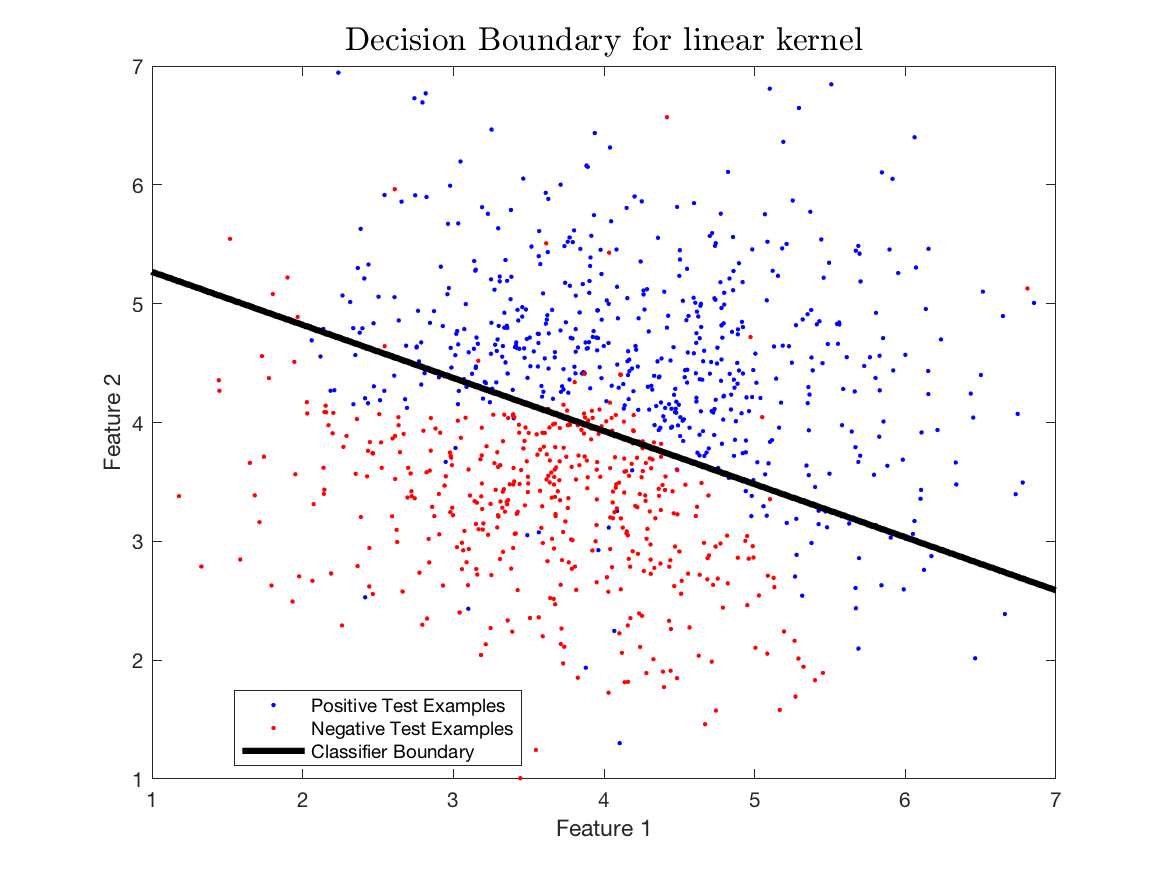
\includegraphics[scale = 0.6]{linear}\newline
\end{figure}

\item Cross Validation Error = 0.0840
\item Training Error = 0.0860
\item Test Error = 0.1090
\end{enumerate}

\pagebreak
\item 
\begin{enumerate}

\item report value of C and insert plot of decision boundary for the rbf-0.1 \newline
$$C = 1$$

\begin{figure}[H]
\centering
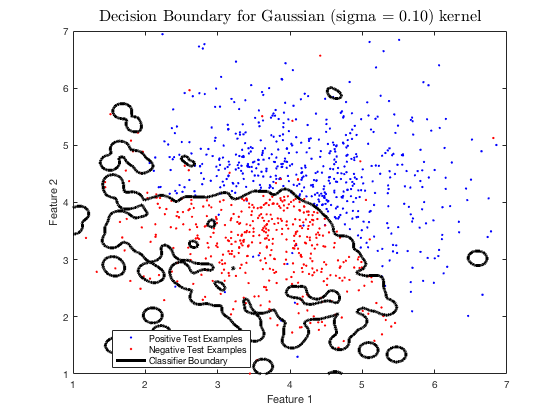
\includegraphics[scale = 0.6]{sig1}\newline
\end{figure}

\item report value of C and insert plot of decision boundary for the rbf-1\newline
$$C = 100$$

\begin{figure}[H]
\centering
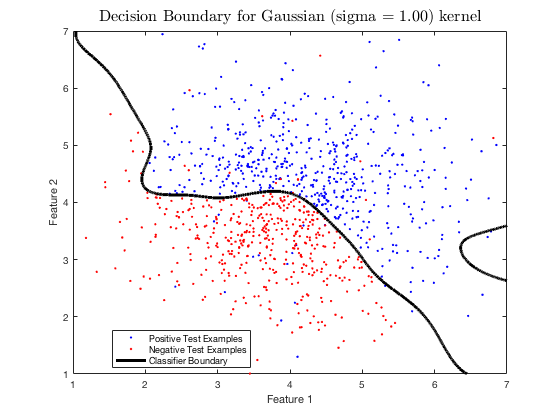
\includegraphics[scale = 0.6]{sig2}\newline
\end{figure}

\item report value of C and insert plot of decision boundary for the rbf-10\newline
$$C = 100000$$

\begin{figure}[H]
\centering
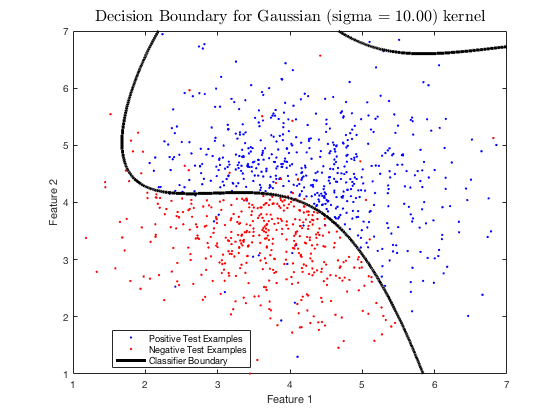
\includegraphics[scale = 0.6]{sig3}\newline
\end{figure}

\item report value of C and insert plot of decision boundary for the rbf-100\newline
$$C = 100000$$

\begin{figure}[H]
\centering
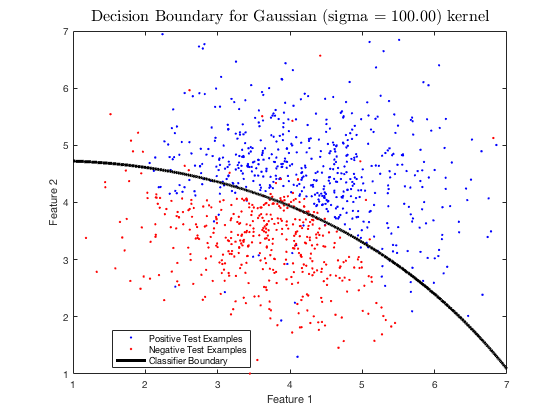
\includegraphics[scale = 0.6]{sig4}\newline
\end{figure}

\item report value of C and insert plot of decision boundary for the rbf-1000 \newline
$$C = 100000$$

\begin{figure}[H]
\centering
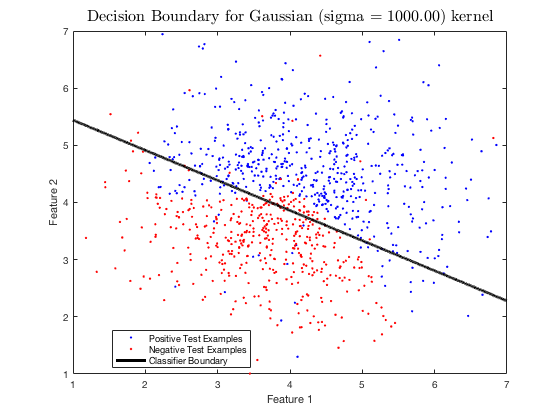
\includegraphics[scale = 0.6]{sig5}\newline
\end{figure}

\item insert line plot of errors \newline

\begin{figure}[H]
\centering
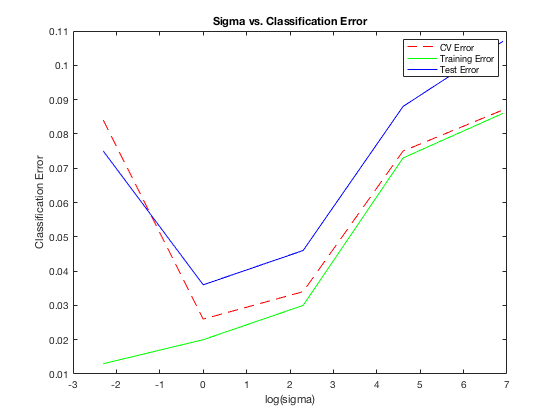
\includegraphics[scale = 0.6]{RBF_error}\newline
\end{figure}

\item $\sigma$ that achieves lowest test error is $\sigma = 1$.
\item $\sigma$ that achieves lowest cross-validation error is $\sigma = 1$
\end{enumerate}
\item 
\begin{enumerate}
\item Absolute difference between test errors is $0$
\item The difference between the two test errors being $0$ makes sense because the cross validation error is a mini version of the overall test error. It is no surprise that it closely follows the trend in the test error. This implies that selecting parameter values using cross-validation is a good approach, since the CV error is a good stand-in for the test error.
\end{enumerate}
\end{enumerate}
\subsection{SVM and Neural Nets on Breast Cancer Dataset}
\begin{enumerate}
    \item Summary of SVM results:
    	For the linear kernel, the smallest cross-validation error value is observed to be $CV-error = 0.0317$. This corresponds to a penalty value of  $C = 1000$. The training error for this model is $training-error = 0.0250$. For the RBF kernel, two pairs of $(sigma, C)$ yield the same cross-validation error. $\sigma = 100$ or $\sigma = 1000$ with $C = 10$ or $C = 1000$ both lead to a CV error of $CV-error = 0.0267$. The pairs also have an identical training error value of $training-error = 0.0267$. The CV error for the RBF kernel is lower than that for the linear kernel, indicating that the RBF kernel potentially outperforms the linear kernel even on test data. The choice between the two candidate RBF kernels can then be made by picking the more complex of the two alternatives. Therefore, an RBF kernel with $\sigma = 1000$ and $C = 1000$ is the best suited SVM model. With this choice of parameters, the SVM produced a test error of $0.02$ in the autograder. 
    \item Summary of NN results: 
    	The neural network can be built with either the ReLU or the sigmoidal activation function, each with a range of penalty ($C$) values. The best penalty for each function can then be selected by using cross-validation. When this approach was used, it was observed that the function and the penalty that yield the lowest cross-validation error are not consistent in different training runs of the neural network. The choice of best $C$ and function that minimizes the CV error keeps changing. The values of the CV error remain fairly close for both kinds of activation functions. Therefore, instead of the CV error, we use the time it takes to train each kind of NN as a metric to pick between the two functions. Alternatively, a random number generator for the initialization that is seeded the same way could be used. However, we determined that training time provided a more intuitive metric. 
	On multiple training runs with both kinds of activation functions, it was observed that neural networks that use the sigmoidal function take longer to train than those that use the ReLU. This is reasonable, since weights in a neural network are learned using back-propagation and gradient descent and it is computationally easier to compute gradients of the ReLU. Therefore, a ReLU activated neural network is a better model compared to a sigmoid activated NN. The choice of C for the ReLU does not seem to affect the CV error in a discernible way. Values of CV error for different C values remain very close to each other. In the neural net that was used to generate the test labels, the ReLU training error was observed to be $0.0667$ and the choice of C was $0.1$. The minimum CV error that corresponded to this C value was $0.6750$. In other runs of the neural network, despite the randomness, these values do not deviate significantly (CV error is always approximately $0.7$ and the training error hovers between $0.03$ and $0.07$ for the ReLU).  
	This ReLU-activated NN produced a test error of $0.06$ is the autograder. 
\end{enumerate}

\subsection{Appendix}
\textbf{Code for 4.2.1 lin-kern-cancer.m}
\color{red}
\begin{verbatim}
clc; close all; clear;


%% Pick a C using CV

C = [1, 10, 10^2, 10^3, 10^4, 10^5];
error = zeros(5, size(C, 2));
cd Breast-Cancer/CrossValidation
% make sure to be in the CrossValidation folder for the loop to work
for i = 1:5
    newFolder = sprintf('Fold%d', i);
    cd(newFolder);
    load('cv-train.mat');
    load('cv-test.mat');
    X = cv_train(:,1:9);
    Y = cv_train(:,10);
    X_test = cv_test(:,1:9);
    Y_test = cv_test(:,10);
    for j = 1:size(C, 2)
        SVMModel = fitcsvm(X, Y, 'BoxConstraint', C(j), 'KernelFunction', 'linear');
        labels_test = predict(SVMModel, X_test);
        % error(i,j) = sum((labels_train - Y_test).^2)/(numel(Y_test));
        % error(i,j) = sum(labels_test ~= Y_test)/(numel(Y_test));
        error(i,j) = classification_error(labels_test, Y_test);
    end
    cd .. % return to CrossValidation from Foldi
end
error_av_CV = mean(error, 1); % this is the cross-validation error
% 10^4 looks to be the smallest
[~, idx] = min(error_av_CV);
error_CV = error_av_CV(idx);
C_choice = C(idx);

%% Use chosen C to train and test
clearvars -except error_av_CV C_choice

cd .. % return to Breast-Cancer
load('trainingdata.mat');
load('testdata.mat');
% X = train(:,1:9);
X = train_inputs;
% Y = train(:,10);
Y = train_labels;
% X_test = test(:,1:9);
X_test = test_inputs;
% Y_test = test(:,10);

SVMModel = fitcsvm(X, Y, 'BoxConstraint', C_choice, 'KernelFunction', 'linear');
labels_train = predict(SVMModel, X); % for training error
% train_error = sum((labels_train - Y).^2)/(numel(Y));
% train_error = sum(labels_train ~= Y)/(numel(Y));
train_error = classification_error(labels_train, Y);

labels_test = predict(SVMModel, X_test); % for testing error
% test_error = sum((labels_test - Y_test).^2)/(numel(Y_test));
% test_error = sum(labels_test ~= Y_test)/(numel(Y_test));

%% Visualize boundary
% cd .. % return to hw4-kit
% decision_boundary_SVM(X_test, Y_test, SVMModel, 1000, 'linear');

%% Helper Function

function err = classification_error(y_pred, y_true)
% This function computes the classification error for the predicted labels
% with respect to the ground truth. The returned error value is a real number
% between 0 and 1 (fraction of misclassications).

% y_true: vector of true labels (each label +1/-1)
% y_pred: vector of predicted labels (each prediction +1/-1)
% err: classification error (fraction of misclassifications)

	err = 1 - length(find(y_pred == y_true)) / length(y_true);
end
\end{verbatim}

\color{black}

\noindent\textbf{Code for 4.2.2: neural-net.m}
\color{red}

\begin{verbatim}
clc; close all; clear;

C = [0, 10^-4, 10^-3, 10^-2, 10^-1, 1];
error = zeros(5, size(C, 2));
cd Breast-Cancer/CrossValidation
% make sure to be in the CrossValidation folder for the loop to work

%% Activation Function: Sigmoid

for i = 1:5
    newFolder = sprintf('Fold%d', i);
    cd(newFolder);
    load('cv-train.mat');
    load('cv-test.mat');
    X = cv_train(:,1:9); % first 9 columns are features
    Y = cv_train(:,10); % 10-th column is labels
    Y(Y == -1) = 0;
    X_test = cv_test(:,1:9);
    Y_test = cv_test(:,10);
    Y_test(Y_test == -1) = 0;
    for j = 1:size(C, 2)
        net = patternnet(10, 'trainrp', 'crossentropy');
        net.layers{1}.transferFcn = 'logsig';
        net.performParam.regularization = C(j);
        net = trainrp(net, X', Y'); 
        labels_pred = net(X_test');
        % labels_pred(labels_pred < 0.5) = 0;
        labels_pred(labels_pred < 0.5) = -1;
        labels_pred(labels_pred > 0.5) = 1;
        labels_pred(labels_pred == 0.5) = 1;
        % error(i,j) = sum(labels_pred' ~= Y_test)/(numel(Y_test));
        error(i,j) = classification_error(labels_pred', Y_test);
    end
    cd .. % return to CrossValidation from Foldi
end
error_av_CV_sig = mean(error, 1); % this is the cross-validation error
% 10^4 looks to be the smallest
[error_min_sig, idx] = min(error_av_CV_sig);
C_choice_sig = C(idx);


%% Activation Function: ReLU

error = zeros(5, size(C, 2)); % reset error matrix
for i = 1:5
    newFolder = sprintf('Fold%d', i);
    cd(newFolder);
    load('cv-train.mat');
    load('cv-test.mat');
    X = cv_train(:,1:9); % first 9 columns are features
    Y = cv_train(:,10); % 10-th column is labels
    Y(Y == -1) = 0;
    X_test = cv_test(:,1:9);
    Y_test = cv_test(:,10);
    Y_test(Y_test == -1) = 0;
    for j = 1:size(C, 2)
        net = patternnet(10, 'trainrp', 'crossentropy');
        net.layers{1}.transferFcn = 'poslin';
        net.performParam.regularization = C(j);
        net = trainrp(net, X', Y'); 
        labels_pred = net(X_test');
        % labels_pred(labels_pred < 0.5) = 0;
        labels_pred(labels_pred < 0.5) = -1;
        labels_pred(labels_pred > 0.5) = 1;
        labels_pred(labels_pred == 0.5) = 1;
        % error(i,j) = sum(labels_pred' ~= Y_test)/(numel(Y_test));
        error(i,j) = classification_error(labels_pred', Y_test);
    end
    cd .. % return to CrossValidation from Foldi
end
error_av_CV_relu = mean(error, 1); % this is the cross-validation error
% 10^4 looks to be the smallest
[error_min_relu, idx] = min(error_av_CV_relu);
C_choice_relu = C(idx);

%% Predictions on Test Inputs
clearvars -except error_av_CV_sig error_min_sig C_choice_sig ...
    error_av_CV_relu error_min_relu C_choice_relu

cd .. % return to Synthetic
load('trainingdata.mat');
load('testdata.mat');
cd .. % return to hw4-kit

% X = train(:,1:9);
X = train_inputs;
% Y = train(:,10);
Y = train_labels;
% X_test = test(:,1:9);
X_test = test_inputs;
% Y_test = test(:,10);

net = patternnet(10, 'trainrp', 'crossentropy');
net.layers{1}.transferFcn = 'logsig';
net.performParam.regularization = C_choice_sig; % chosen C for sigmoid act.
net = trainrp(net, X', Y'); 
labels_pred_sig = net(X_test');
% labels_pred_sig(labels_pred_sig < 0.5) = 0;
labels_pred_sig(labels_pred_sig < 0.5) = -1;
labels_pred_sig(labels_pred_sig > 0.5) = 1;
labels_pred_sig(labels_pred_sig == 0.5) = 1;

% for training error
labels_train_sig = net(X'); % run neural net on training data
% labels_train_sig(labels_train_sig < 0.5) = 0;
labels_train_sig(labels_train_sig < 0.5) = -1;
labels_train_sig(labels_train_sig > 0.5) = 1;
labels_train_sig(labels_train_sig == 0.5) = 1;
% train_error_sig = sum(labels_train_sig' ~= Y)/(numel(Y));
train_error_sig = classification_error(labels_train_sig', Y);

net = patternnet(10, 'trainrp', 'crossentropy');
net.layers{1}.transferFcn = 'poslin';
net.performParam.regularization = C_choice_relu; % chosen C for ReLU act.
net = trainrp(net, X', Y'); 
labels_pred_relu = net(X_test');
% labels_pred_relu(labels_pred_relu < 0.5) = 0;
labels_pred_relu(labels_pred_relu < 0.5) = -1;
labels_pred_relu(labels_pred_relu > 0.5) = 1;
labels_pred_relu(labels_pred_relu == 0.5) = 1;

% for training error
labels_train_relu = net(X'); % run neural net on training data
% labels_train_relu(labels_train_relu < 0.5) = 0;
labels_train_relu(labels_train_relu < 0.5) = -1;
labels_train_relu(labels_train_relu > 0.5) = 1;
labels_train_relu(labels_train_relu == 0.5) = 1;
% train_error_relu = sum(labels_train_relu' ~= Y)/(numel(Y));
train_error_relu = classification_error(labels_train_relu', Y);

%% Helper Function

function err = classification_error(y_pred, y_true)
% This function computes the classification error for the predicted labels
% with respect to the ground truth. The returned error value is a real number
% between 0 and 1 (fraction of misclassications).

% y_true: vector of true labels (each label +1/-1)
% y_pred: vector of predicted labels (each prediction +1/-1)
% err: classification error (fraction of misclassifications)

	err = 1 - length(find(y_pred == y_true)) / length(y_true);
end
\end{verbatim}
\end{document}
